\documentclass[tikz,border=2pt,10pt]{standalone}
\usepackage[T1]{fontenc}
\usepackage{lmodern,amsmath,amssymb}
\usetikzlibrary{arrows.meta,calc,backgrounds}
\definecolor{ink}{RGB}{31,40,48}
\definecolor{uclr}{RGB}{155,72,28}
\definecolor{tclr}{RGB}{29,84,126}
\definecolor{res}{RGB}{20,101,84}
\begin{document}
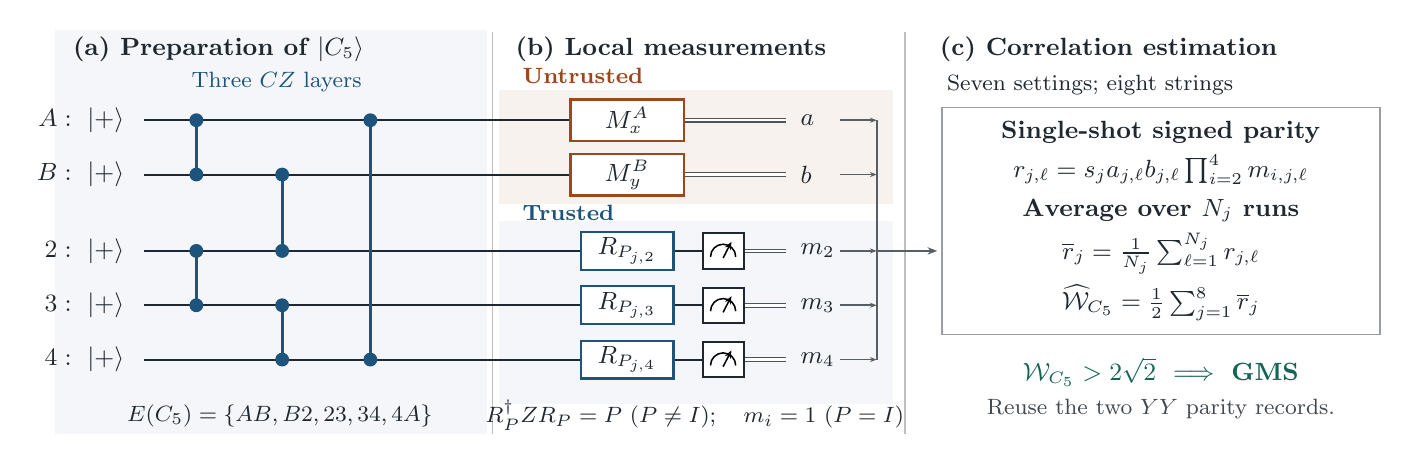
\begin{tikzpicture}[x=1cm,y=1cm,font=\small,text=ink,
wire/.style={draw=ink,line width=.7pt},
cz/.style={draw=tclr,line width=1pt},
dot/.style={circle,fill=tclr,inner sep=0pt,minimum size=5pt},
blackbox/.style={draw=uclr,fill=white,line width=.85pt,minimum width=1.44cm,minimum height=.53cm,inner sep=2pt},
rotation/.style={draw=tclr,fill=white,line width=.75pt,minimum width=1.18cm,minimum height=.48cm,inner sep=1pt},
meter/.style={draw=ink,fill=white,line width=.7pt,minimum width=.52cm,minimum height=.45cm,inner sep=0pt},
classical/.style={draw=ink!80,double,double distance=.9pt,line width=.42pt},
head/.style={font=\small\bfseries,anchor=west},
smallnote/.style={font=\footnotesize,align=center}]
% Panel titles and subtle regions; no heavy frames.
\fill[tclr!5] (.0,-.35) rectangle (5.48,4.78);
\fill[uclr!7] (5.63,2.57) rectangle (10.64,4.02);
\fill[tclr!5] (5.63,.02) rectangle (10.64,2.35);
\node[head] at (.10,4.53) {(a) Preparation of $|C_5\rangle$};
\node[head] at (5.72,4.53) {(b) Local measurements};
\node[head] at (11.11,4.53) {(c) Correlation estimation};
\draw[ink!30,line width=.45pt] (5.55,-.35)--(5.55,4.75);
\draw[ink!30,line width=.45pt] (10.79,-.35)--(10.79,4.75);
% Preparation: disjoint CZs can be placed in a common gate layer.
\foreach \q/\y in {A/3.63,B/2.94,2/1.97,3/1.28,4/.59}{
 \node[anchor=east] at (1.00,\y) {$\q:\ |+\rangle$};
 \draw[wire] (1.13,\y)--(6.44,\y);
}
\foreach \x/\ya/\yb in {1.79/3.63/2.94,1.79/1.97/1.28,2.88/2.94/1.97,2.88/1.28/.59,4.00/3.63/.59}{
 \draw[cz] (\x,\ya)--(\x,\yb);
 \node[dot] at (\x,\ya) {};
 \node[dot] at (\x,\yb) {};
}
\node[smallnote,text=tclr] at (2.81,4.11) {Three $CZ$ layers};
\node[smallnote] at (2.85,-.12) {$E(C_5)=\{AB,B2,23,34,4A\}$};
% Black boxes: the settings are classical inputs, internal operations unknown.
\node[font=\footnotesize\bfseries,text=uclr,anchor=west] at (5.81,4.20) {Untrusted};
\node[blackbox] (A) at (7.26,3.63) {$M^A_x$};
\node[blackbox] (B) at (7.26,2.94) {$M^B_y$};
\foreach \n/\y/\o/\s in {A/3.63/a/x,B/2.94/b/y}{
 \draw[wire] (6.44,\y)--(\n.west);
 \draw[classical] (\n.east)--(9.28,\y);
 \node[anchor=west] at (9.34,\y) {$\o$};
}
% Trusted laboratories: local basis rotation and Z readout.
\node[font=\footnotesize\bfseries,text=tclr,anchor=west] at (5.81,2.45) {Trusted};
\foreach \q/\y in {2/1.97,3/1.28,4/.59}{
 \node[rotation] (R\q) at (7.26,\y) {$R_{P_{j,\q}}$};
 \node[meter] (D\q) at (8.48,\y) {};
 \draw[wire] (6.44,\y)--(R\q.west);
 \draw[wire] (R\q.east)--(D\q.west);
 \draw[line width=.55pt] ($(D\q.center)+(-.16,-.075)$) arc[start angle=180,end angle=0,radius=.16cm];
 \draw[-{Stealth[length=2.8pt,width=2.4pt]},line width=.55pt] ($(D\q.center)+(0,-.09)$)--($(D\q.center)+(.105,.115)$);
 \draw[classical] (D\q.east)--(9.28,\y);
 \node[anchor=west] at (9.34,\y) {$m_{\q}$};
}
\node[smallnote] at (8.12,-.12) {$R_P^\dagger ZR_P=P\ (P\ne I);\quad m_i=1\ (P=I)$};
% Classical collection bus; records are combined only after readout.
\foreach \y in {3.63,2.94,1.97,1.28,.59}{
 \draw[ink!75,line width=.55pt,-{Stealth[length=2.4pt]}] (9.96,\y)--(10.43,\y);
}
\draw[ink!75,line width=.65pt] (10.43,.59)--(10.43,3.63);
\draw[ink!75,line width=.8pt,-{Stealth[length=3.5pt]}] (10.43,1.97)--(11.20,1.97);
% Estimator: distinguish each single-shot record from correlator averages.
\node[smallnote,anchor=west] at (11.20,4.08) {Seven settings; eight strings};
\node[draw=ink!45,line width=.65pt,fill=white,align=center,inner sep=5pt,minimum width=5.57cm,minimum height=2.45cm] at (14.04,2.35) {
 \textbf{Single-shot signed parity}\\[3pt]
 $r_{j,\ell}=s_j a_{j,\ell} b_{j,\ell}\prod_{i=2}^{4}m_{i,j,\ell}$\\[3pt]
 \textbf{Average over $N_j$ runs}\\[3pt]
 $\overline r_j=\frac{1}{N_j}\sum_{\ell=1}^{N_j}r_{j,\ell}$\\[3pt]
 $\widehat{\mathcal W}_{C_5}=\frac12\sum_{j=1}^{8}\overline r_j$
};
\node[font=\small\bfseries,text=res] at (14.04,.43) {$\mathcal W_{C_5}>2\sqrt2\ \Longrightarrow\ \text{GMS}$};
\node[smallnote,text=ink!85] at (14.04,-.04) {Reuse the two $YY$ parity records.};
\end{tikzpicture}
\end{document}
